  \vspace{-3mm}
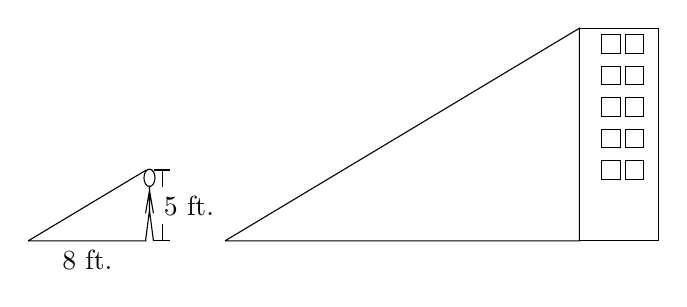
\begin{tikzpicture}
\draw (0,0)--(1.5,0)(1.5,0.9)--(0,0);
\draw (1.54,0.8) ellipse (.07 cm and .11 cm);
\draw(1.54,0.7)--(1.54,0.39)--(1.49,0)
(1.54,0.39)--(1.59,0)
(1.54,.64)--(1.49,0.35)
(1.54,.64)--(1.59,.35);
\draw(1.7,0)--(1.7,0.9)(1.6,0.9)--(1.8,0.9)(1.6,0)--(1.8,0);
\draw (1.6,0.45)node[anchor=west, rectangle, fill=white]{5 ft.} (0.75,0)node[anchor=north]{8 ft.};
\draw(2.5,0)--(7,0)--(7,2.7)--(2.5,0);
\draw(7,0)--(8,0)--(8,2.7)--(7,2.7);
\foreach \i in {7.4, 7.7}
\foreach \j in {0.9, 1.3, 1.7, 2.1, 2.5}
\draw(\i,\j)node[shape=rectangle, text=white, draw=black]{};;
\end{tikzpicture}\\
The diagrams above, drawn to different scales, represent the measurement of two shadows.  One of the shadows belongs to a teenager standing orthagonal to the ground, and the other is of an edifice that is likewise at a right angle to the ground.  As the shadows are measured at the same time there is no observable difference between the corresponding angles on the ground.  If the building's shadow is measured to be $280$ feet, what is the building's height?  Grid your answer in terms of feet.\\



\ifsat
	\begin{enumerate}[label=\Alph*)]
	\end{enumerate}
\else
\fi

\ifacteven
	\begin{enumerate}[label=\textbf{\Alph*.},itemsep=\fill,align=left]
		\setcounter{enumii}{5}
		\item None of these. 
	\end{enumerate}
\else
\fi

\ifactodd
	\begin{enumerate}[label=\textbf{\Alph*.},itemsep=\fill,align=left]
		\item None of these. 
	\end{enumerate}
\else
\fi

\ifgridin
$175$ feet
\else
\fi

